\documentclass[onlymath]{beamer}
% \documentclass[onlymath,handout]{beamer}

% Macros used by all lectures, but not necessarily by excercises

%%% General setup and dependencies:

% \usetheme[ddcfooter,nosectionnum]{tud}
\usetheme[nosectionnum,pagenum,noheader]{tud}
% \usetheme[nosectionnum,pagenum]{tud}

% Increase body font size to a sane level:
\let\origframetitle\frametitle
% \renewcommand{\frametitle}[1]{\origframetitle{#1}\normalsize}
\renewcommand{\frametitle}[1]{\origframetitle{#1}\fontsize{10pt}{13.2}\selectfont}
\setbeamerfont{itemize/enumerate subbody}{size=\small} % tud defaults to scriptsize!
\setbeamerfont{itemize/enumerate subsubbody}{size=\small}
% \setbeamerfont{normal text}{size=\small}
% \setbeamerfont{itemize body}{size=\small}

\renewcommand{\emph}[1]{\textbf{#1}}

\def\arraystretch{1.3}% Make tables even less cramped vertically

\usepackage[ngerman]{babel}
\usepackage[utf8]{inputenc}
\usepackage[T1]{fontenc}

%\usepackage{graphicx}
\usepackage[export]{adjustbox} % loads graphicx
\usepackage{import}
\usepackage{stmaryrd}
\usepackage[normalem]{ulem} % sout command
% \usepackage{times}
\usepackage{txfonts}

% \usepackage[perpage]{footmisc} % reset footnote counter on each page -- fails with beamer (footnotes gone)
\usepackage{perpage}  % reset footnote counter on each page
\MakePerPage{footnote}

\usepackage{tikz}
\usetikzlibrary{arrows,positioning}
% Inspired by http://www.texample.net/tikz/examples/hand-drawn-lines/
\usetikzlibrary{decorations.pathmorphing}
\pgfdeclaredecoration{penciline}{initial}{
    \state{initial}[width=+\pgfdecoratedinputsegmentremainingdistance,
    auto corner on length=1mm,]{
        \pgfpathcurveto%
        {% From
            \pgfqpoint{\pgfdecoratedinputsegmentremainingdistance}
                      {\pgfdecorationsegmentamplitude}
        }
        {%  Control 1
        \pgfmathrand
        \pgfpointadd{\pgfqpoint{\pgfdecoratedinputsegmentremainingdistance}{0pt}}
                    {\pgfqpoint{-\pgfdecorationsegmentaspect
                     \pgfdecoratedinputsegmentremainingdistance}%
                               {\pgfmathresult\pgfdecorationsegmentamplitude}
                    }
        }
        {%TO 
        \pgfpointadd{\pgfpointdecoratedinputsegmentlast}{\pgfpoint{1pt}{1pt}}
        }
    }
    \state{final}{}
}
\tikzset{handdrawn/.style={decorate,decoration=penciline}}
\tikzset{every shadow/.style={fill=none,shadow xshift=0pt,shadow yshift=0pt}}
% \tikzset{module/.append style={top color=\col,bottom color=\col}}

% Use to make Tikz attributes with Beamer overlays
% http://tex.stackexchange.com/a/6155
\tikzset{onslide/.code args={<#1>#2}{%
  \only<#1| handout:0>{\pgfkeysalso{#2}} 
}}
\tikzset{onslideprint/.code args={<#1>#2}{%
  \only<#1>{\pgfkeysalso{#2}} 
}}

%%% Title -- always set this first

\newcommand{\defineTitle}[3]{
	\newcommand{\lectureindex}{#1}
	\title{Formale Systeme}
	\subtitle{\href{\lectureurl}{#1. Vorlesung: #2}}
	\author{\href{http://korrekt.org/}{Markus Kr\"{o}tzsch}}
%	\author{\href{http://www.sebastian-rudolph.de}{Sebastian Rudolph} in Vertretung von \href{http://korrekt.org/}{Markus Kr\"{o}tzsch}}
	\date{#3}
	\datecity{TU Dresden}
% 	\institute{Computational Logic}
}

%%% Table of contents:

\RequirePackage{ifthen}

\newcommand{\highlight}[2]{%
	\ifthenelse{\equal{#1}{\lectureindex}}{\alert{#2}}{#2}%
}

\def\myspace{-0.7ex}
\newcommand{\printtoc}{
\begin{tabular}{r@{$\quad$}l}
\highlight{1}{1.} & \highlight{1}{Willkommen/Einleitung formale Sprachen}\\[\myspace]
\highlight{2}{2.} & \highlight{2}{Grammatiken und die Chomsky-Hierarchie}\\[\myspace]
\highlight{3}{3.} & \highlight{3}{Endliche Automaten}\\[\myspace]
\highlight{4}{4.} & \highlight{4}{Complexity of FO query answering}\\[\myspace]
\highlight{5}{5.} & \highlight{5}{Conjunctive queries}\\[\myspace]
\highlight{6}{6.} & \highlight{6}{Tree-like conjunctive queries}\\[\myspace]
\highlight{7}{7.} & \highlight{7}{Query optimisation}\\[\myspace]
\highlight{8}{8.} & \highlight{8}{Conjunctive Query Optimisation / First-Order~Expressiveness}\\[\myspace]
\highlight{9}{9.} & \highlight{9}{First-Order~Expressiveness / Introduction to Datalog}\\[\myspace]
\highlight{10}{10.} & \highlight{10}{Expressive Power and Complexity of Datalog}\\[\myspace]
\highlight{11}{11.} & \highlight{11}{Optimisation and Evaluation of Datalog}\\[\myspace]
\highlight{12}{12.} & \highlight{12}{Evaluation of Datalog (2)}\\[\myspace]
\highlight{13}{13.} & \highlight{13}{Graph Databases and Path Queries}\\[\myspace]
\highlight{14}{14.} & \highlight{14}{Outlook: database theory in practice}
\end{tabular}
}

\newcommand{\overviewslide}{%
\begin{frame}\frametitle{Overview}
\printtoc
\medskip

Siehe \href{\lectureurl}{course homepage [$\Rightarrow$ link]} for more information and materials
\end{frame}
}

%%% Colours:

\usepackage{xcolor,colortbl}
\definecolor{redhighlights}{HTML}{FFAA66}
\definecolor{lightblue}{HTML}{55AAFF}
\definecolor{lightred}{HTML}{FF5522}
\definecolor{lightpurple}{HTML}{DD77BB}
\definecolor{lightgreen}{HTML}{55FF55}
\definecolor{darkred}{HTML}{CC4411}
\definecolor{darkblue}{HTML}{176FC0}%{1133AA}
\definecolor{nightblue}{HTML}{2010A0}%{1133AA}
\definecolor{alert}{HTML}{176FC0}
\definecolor{darkgreen}{HTML}{36AB14}
\definecolor{strongyellow}{HTML}{FFE219}
\definecolor{devilscss}{HTML}{666666}

\newcommand{\redalert}[1]{\textcolor{darkred}{#1}}

%%% Style commands

\newcommand{\quoted}[1]{\texttt{"}{#1}\texttt{"}}
\newcommand{\squote}{\texttt{"}} % straight quote
\newcommand{\Sterm}[1]{\ensuremath{\mathtt{\textcolor{purple}{#1}}}}    % letters in alphabets
\newcommand{\Snterm}[1]{\textsf{\textcolor{darkblue}{#1}}} % nonterminal symbols
\newcommand{\Sntermsub}[2]{\Snterm{#1}_{\Snterm{#2}}} % nonterminal symbols
\newcommand{\Slang}[1]{\textbf{\textcolor{black}{#1}}}    % languages
\newcommand{\Slangsub}[2]{\Slang{#1}_{\Slang{#2}}}    % languages
% Code
\newcommand{\Scode}[1]{\textbf{#1}}    % reserved words in program listings, e.g., "if"
\newcommand{\Scodelit}[1]{\textcolor{purple}{#1}}    % literals in program listings, e.g., strings
\newcommand{\Scomment}[1]{\textcolor{gray}{#1}}    % comment in program listings

\newcommand{\epstrastar}{\mathrel{\mathord{\stackrel{\epsilon}{\to}}{}^*}} % transitive reflexive closure of epsilon transitions in an epslion-NFA

\newcommand{\narrowcentering}[1]{\mbox{}\hfill#1\hfill\mbox{}}

\newcommand{\defeq}{\mathrel{:=}}

\newcommand{\Smach}[1]{\ensuremath{\mathcal{#1}}}    % machines

%%% Slide layout commands:

\newcommand{\sectionSlide}[1]{
\frame{\begin{center}
\LARGE
#1
\end{center}}
}
\newcommand{\sectionSlideNoHandout}[1]{
\frame<handout:0>{\begin{center}
\LARGE
#1
\end{center}}
}

\newcommand{\mydualbox}[3]{%
 \begin{minipage}[t]{#1}
 \begin{beamerboxesrounded}[upper=block title,lower=block body,shadow=true]%
    {\centering\usebeamerfont*{block title}#2}%
    \raggedright%
    \usebeamerfont{block body}
%     \small
    #3%
  \end{beamerboxesrounded}
  \end{minipage}
}
% 
\newcommand{\myheaderbox}[2]{%
 \begin{minipage}[t]{#1}
 \begin{beamerboxesrounded}[upper=block title,lower=block title,shadow=true]%
    {\centering\usebeamerfont*{block title}\rule{0pt}{2.6ex} #2}%
  \end{beamerboxesrounded}
  \end{minipage}
}

\newcommand{\mycontentbox}[2]{%
 \begin{minipage}[t]{#1}%
 \begin{beamerboxesrounded}[upper=block body,lower=block body,shadow=true]%
    {\centering\usebeamerfont*{block body}\rule{0pt}{2.6ex}#2}%
  \end{beamerboxesrounded}
  \end{minipage}
}

\newcommand{\mylcontentbox}[2]{%
 \begin{minipage}[t]{#1}%
 \begin{beamerboxesrounded}[upper=block body,lower=block body,shadow=true]%
    {\flushleft\usebeamerfont*{block body}\rule{0pt}{2.6ex}#2}%
  \end{beamerboxesrounded}
  \end{minipage}
}

% label=180:{\rotatebox{90}{{\footnotesize\textcolor{darkgreen}{Beispiel}}}}
% \hspace{-8mm}\ghost{\raisebox{-7mm}{\rotatebox{90}{{\footnotesize\textcolor{darkgreen}{Beispiel}}}}}\hspace{8mm}
\newcommand{\examplebox}[1]{%
	\begin{tikzpicture}[decoration=penciline, decorate]
		\pgfmathsetseed{1235}
		\node (n1) [decorate,draw=darkgreen, fill=darkgreen!10,thick,align=left,text width=\linewidth, inner ysep=2mm, inner xsep=2mm] at (0,0) {#1};
% 		\node (n2) [align=left,text width=\linewidth,inner sep=0mm] at (n1.92) {{\footnotesize\raisebox{3mm}{\textcolor{darkgreen}{Beispiel}}}};
% 		\node (n2) [decorate,draw=darkgreen, fill=darkgreen!10,thick, align=left,text width=\linewidth,inner sep=2mm] at (n1.90) {{\footnotesize\raisebox{0mm}{\textcolor{darkgreen}{Beispiel}}}};
	\end{tikzpicture}%
}%

\newcommand{\codebox}[1]{%
	\begin{tikzpicture}[decoration=penciline, decorate]
		\pgfmathsetseed{1236}
		\node (n1) [decorate,draw=strongyellow, fill=strongyellow!10,thick,align=left,text width=\linewidth, inner ysep=2mm, inner xsep=2mm] at (0,0) {#1};
	\end{tikzpicture}%
}%

\newcommand{\defbox}[1]{%
	\begin{tikzpicture}[decoration=penciline, decorate]
		\pgfmathsetseed{1237}
		\node (n1) [decorate,draw=darkred, fill=darkred!10,thick,align=left,text width=\linewidth, inner ysep=2mm, inner xsep=2mm] at (0,0) {#1};
	\end{tikzpicture}%
}%

\newcommand{\theobox}[1]{%
	\begin{tikzpicture}[decoration=penciline, decorate]
		\pgfmathsetseed{1240}
		\node (n1) [decorate,draw=darkblue, fill=darkblue!10,thick,align=left,text width=\linewidth, inner ysep=2mm, inner xsep=2mm] at (0,0) {#1};
	\end{tikzpicture}%
}%

\newcommand{\anybox}[2]{%
	\begin{tikzpicture}[decoration=penciline, decorate]
		\pgfmathsetseed{1240}
		\node (n1) [decorate,draw=#1, fill=#1!10,thick,align=left,text width=\linewidth, inner ysep=2mm, inner xsep=2mm] at (0,0) {#2};
	\end{tikzpicture}%
}%


\newsavebox{\mybox}%
\newcommand{\doodlebox}[2]{%
\sbox{\mybox}{#2}%
	\begin{tikzpicture}[decoration=penciline, decorate]
		\pgfmathsetseed{1238}
		\node (n1) [decorate,draw=#1, fill=#1!10,thick,align=left,inner sep=1mm] at (0,0) {\usebox{\mybox}};
	\end{tikzpicture}%
}%

% Common notation

\usepackage{amsmath,amssymb,amsfonts}
\usepackage{xspace}

\newcommand{\lectureurl}{https://iccl.inf.tu-dresden.de/web/FS2016}

\DeclareMathAlphabet{\mathsc}{OT1}{cmr}{m}{sc} % Let's have \mathsc since the slide style has no working \textsc

% Dual of "phantom": make a text that is visible but intangible
\newcommand{\ghost}[1]{\raisebox{0pt}[0pt][0pt]{\makebox[0pt][l]{#1}}}

\newcommand{\tuple}[1]{\langle{#1}\rangle}

%%% Annotation %%%

\usepackage{color}
\newcommand{\todo}[1]{{\tiny\color{red}\textbf{TODO: #1}}}



%%% Old macros below; move when needed

\newcommand{\blank}{\text{\textvisiblespace}} % empty tape cell for TM

% table syntax
\newcommand{\dom}{\textbf{dom}}
\newcommand{\adom}{\textbf{adom}}
\newcommand{\dbconst}[1]{\texttt{"#1"}}
\newcommand{\pred}[1]{\textsf{#1}}
\newcommand{\foquery}[2]{#2[#1]}
\newcommand{\ground}[1]{\textsf{ground}(#1)}
% \newcommand{\foquery}[2]{\{#1\mid #2\}} %% Notation as used in Alice Book
% \newcommand{\foquery}[2]{\tuple{#1\mid #2}}

\newcommand{\quantor}{\mathord{\reflectbox{$\text{\sf{Q}}$}}} % the generic quantor

% logic syntax
\newcommand{\Inter}{\mathcal{I}} %used to denote an interpretation
\newcommand{\Jnter}{\mathcal{J}} %used to denote another interpretation
\newcommand{\Knter}{\mathcal{K}} %used to denote yet another interpretation
\newcommand{\Zuweisung}{\mathcal{Z}} %used to denote a variable assignment

% query languages
\newcommand{\qlang}[1]{{\sf #1}} % Font for query languages
\newcommand{\qmaps}[1]{\textbf{QM}({\sf #1})} % Set of query mappings for a query language

%%% Complexities %%%

\hyphenation{Exp-Time} % prevent "Ex-PTime" (see, e.g. Tobies'01, Glimm'07 ;-)
\hyphenation{NExp-Time} % better that than something else

% \newcommand{\complclass}[1]{{\sc #1}\xspace} % font for complexity classes
\newcommand{\complclass}[1]{\ensuremath{\mathsc{#1}}\xspace} % font for complexity classes

\newcommand{\ACzero}{\complclass{AC$_0$}}
\newcommand{\LogSpace}{\complclass{L}}
\newcommand{\NLogSpace}{\complclass{NL}}
\newcommand{\PTime}{\complclass{P}}
\newcommand{\NP}{\complclass{NP}}
\newcommand{\coNP}{\complclass{coNP}}
\newcommand{\PH}{\complclass{PH}}
\newcommand{\PSpace}{\complclass{PSpace}}
\newcommand{\NPSpace}{\complclass{NPSpace}}
\newcommand{\ExpTime}{\complclass{ExpTime}}
\newcommand{\NExpTime}{\complclass{NExpTime}}
\newcommand{\ExpSpace}{\complclass{ExpSpace}}
\newcommand{\TwoExpTime}{\complclass{2ExpTime}}
\newcommand{\NTwoExpTime}{\complclass{N2ExpTime}}
\newcommand{\ThreeExpTime}{\complclass{3ExpTime}}
\newcommand{\kExpTime}[1]{\complclass{#1ExpTime}}
\newcommand{\kExpSpace}[1]{\complclass{#1ExpSpace}}


% \usetikzlibrary{shapes}

\defineTitle{17}{Deterministische Sprachen / Entscheidungsprobleme}{12. Dezember 2016}

\begin{document}

\maketitle

\sectionSlideNoHandout{Rückblick}

\begin{frame}[fragile]\frametitle{PDA ${}\hat{=}{}$ CFG ${}\hat{=}{}$ Typ 2}

% \theobox{Satz: Eine Sprache ist genau dann kontextfrei wenn sie von einem PDA akzeptiert wird.}\bigskip

\begin{tikzpicture}[
	decoration=penciline, decorate,
	node distance = 7mm and 9mm,
	mybox/.style args = {#1/#2}{
		draw=#1,% line color
		fill=#2,% fill color
% 		rounded corners,
		thick,
		text width=18mm, minimum height=12mm, inner sep=1mm,
		align=flush center
	},
	myboxlabel/.style args = {}{
		draw=devilscss,% line color
		fill=strongyellow!40,% fill color
% 		rounded corners,
		thick,
		text width=17mm, minimum height=10mm, inner sep=1.5mm,
		align=flush center
	},
	myarrow/.style args = {#1}{
		line width=0.8mm,
		draw=#1,%line color
		%-{Triangle[length=2.8mm,width=4mm,fill=#1]},
		->,
		shorten >=0.5mm, shorten <=0.1mm
	}
]
\pgfmathsetseed{7729}
% \draw[help lines] (0,0) grid (5,5);
\node (cfg) [decorate,mybox=black/cyan!40] at (0,0) {CFG};
\node (pda) [decorate,mybox=black/cyan!40] at (8,0) {PDA};
\node (gpda) [decorate,mybox=black/cyan!40,text width=28mm] at (4,2) {PDA\\{\footnotesize mit Wort-\texttt{push}}};
\node (spda) [decorate,mybox=black/cyan!40,text width=38mm] at (4,-2) {PDA\vspace{-1.5ex}\begin{flushleft}\tiny
~--~~je ein Start- und ein Endzustand\\
~--~~Keller wird vor Akzeptanz geleert\\
~--~~pro Schritt \texttt{pop} oder \texttt{push}, nie beides\end{flushleft}
};
%
\path[myarrow=devilscss,bend left=20,-](cfg.90) edge[->] (gpda.180);
	\node (cfggpdalabel) [decorate,myboxlabel=,text width=26mm] at (0.2,2.4) {\footnotesize"`$\Snterm{A} \to w$"' $\leadsto$ "`$\tuple{q_l,w}\in\delta(q_l,\epsilon,\Snterm{A})$"'};
\path[myarrow=devilscss,bend left=20,-](gpda.0) edge[->] (pda.90);
	\node (gpdapdalabel) [decorate,myboxlabel=,text width=31mm] at (7.5,2.6) {\footnotesize"`\texttt{push}($\Sntermsub{B}{1}\cdots\Sntermsub{B}{n}$)"' $\leadsto$ "`\texttt{push}($\Sntermsub{B}{n}$),\ldots,\texttt{push}($\Sntermsub{B}{1}$)"'};
\path[myarrow=devilscss,bend left=20,-](pda.270) edge[->] (spda.0);
	\node (gpdapdalabel) [decorate,myboxlabel=,text width=22mm] at (7.8,-2.5) {\footnotesize wie in Vorlesung skizziert};
\path[myarrow=devilscss,bend left=20,-](spda.180) edge[->] (cfg.270);
	\node (spdacfglabel) [decorate,myboxlabel=,text width=19mm] at (-0.1,-2.4) {\footnotesize%
	$\Sntermsub{V}{q,r} \to \Sterm{a}\Sntermsub{V}{s,t}\Sterm{b}$\\
	$\Sntermsub{V}{q,r} \to \Sntermsub{V}{q,s}\Sntermsub{V}{s,r}$\\[-0.7mm]
	$\Sntermsub{V}{q,q} \to \epsilon$};

\node (thm) [decorate,draw=darkblue, fill=darkblue!10,thick,align=left,text width=40mm, inner ysep=2mm, inner xsep=2mm] at (4,0) {Satz: Eine Sprache ist genau dann kontextfrei wenn sie von einem PDA akzeptiert wird.};
\end{tikzpicture}

\end{frame}

\begin{frame}\frametitle{Deterministische Kellerautomaten}

\defbox{Ein \redalert{deterministischer Kellerautomat} (international: "`\alert{DPDA}"') 
\Smach{M} ist ein Tupel $\Smach{M}=\tuple{Q,\Sigma,\Gamma,\delta,q_0,F}$ bestehend aus
{Zustandsmenge} $Q$, {Eingabealphabet} $\Sigma$, {Kelleralphabet} $\Gamma$,
{Startzustand} $q_0\in Q$, {Endzustände} $F\subseteq Q$
und {partieller Übergangsfunktion}\\[1ex]
\narrowcentering{$Q\times\Sigma_\epsilon\times\Gamma_\epsilon \to Q\times\Gamma_\epsilon$,}\\[1ex]
so dass für alle $q\in Q$, $\Sterm{a}\in\Sigma$ und $\Snterm{A}\in\Gamma$
jeweils nur eines der folgenden definiert ist:\\[1ex]
\narrowcentering{$\delta(q,\Sterm{a},\Snterm{A})$\hfill$\delta(q,\Sterm{a},\epsilon)$\hfill$\delta(q,\epsilon,\Snterm{A})$\hfill$\delta(q,\epsilon,\epsilon)$}
}\medskip

Beispiel: $\Sterm{a}^i\Sterm{b}^i$

\narrowcentering{\begin{tikzpicture}[xscale=0.85,baseline={([yshift=-2ex]current bounding box.north)}]
% \draw[help lines] (0,0) grid (7,2);
\node (s) [circle,draw=black,thick,double] at (0,0) {$q_s$};
\node (a) [circle,draw=black,thick] at (3,0) {$q_a$};
\node (b) [circle,draw=black,thick] at (6,0) {$q_b$};
\node (f) [circle,draw=black,thick,double] at (9,0) {$q_f$};
%
\path[->,line width=0.5mm](-1,0) edge (s);
\path[->,line width=0.5mm](s) edge node[above] {$\epsilon,\epsilon\mapsto\Snterm{S}$} (a);
\path[->,line width=0.5mm](a) edge [loop above] node[above] {$\Sterm{a},\epsilon\mapsto\Snterm{A}$} (a);
\path[->,line width=0.5mm](a) edge node[above] {$\Sterm{b},\Snterm{A}\mapsto\epsilon$} (b);
\path[->,line width=0.5mm](b) edge [loop above] node[above] {$\Sterm{b},\Snterm{A}\mapsto\epsilon$} (b);
\path[->,line width=0.5mm](b) edge node[above] {$\epsilon,\Snterm{S}\mapsto\epsilon$} (f);
\end{tikzpicture}}

\end{frame}

\begin{frame}[t]\frametitle{Deterministisch vs. nichtdeterminitisch}

\begin{minipage}[t]{4.7cm}
~~~~\emph{Typ-2-Sprachen}\\
\begin{itemize}
\item Erkannt durch PDAs
\item Nicht unter Komplement abgeschlossen
\item Echte Obermenge der det. Typ-2-Sprachen, z.B. $\{\Sterm{a}^i\Sterm{b}^j\Sterm{c}^k\mid i\neq j \text{ oder }j\neq k\}$
\item Wortproblem in $O(|w|^3)$ (CYK-Algorithmus)
\item Generiert durch CFGs
\end{itemize}
\end{minipage}
\begin{minipage}[t]{4.7cm}
~~~~\emph{Deterministische}\\
\mbox{}~~~~\emph{Typ-2-Sprachen}
\begin{itemize}
\item Erkannt durch DPDAs
\item Unter Komplement abgeschlossen
\item Echte Obermenge der regulären Sprachen, z.B. $\{\Sterm{a}^i\Sterm{b}^i\mid i\geq 0\}$
\item Wortproblem in $O(|w|)$ (DPDA-Abarbeitung)
\item Generiert durch deterministische CFGs (kein Vorlesungsstoff)
\end{itemize}
\end{minipage}

\end{frame}

\sectionSlide{Deterministische Typ-2-Sprachen}


\begin{frame}\frametitle{Rückblick: Ableitungsbäume}

\begin{minipage}[t]{4cm}
\begin{flushleft}
\emph{Rückblick:}\\ Die Interpretation von Wörtern kontextfreier Sprachen
basiert zumeist auf dem Syntaxbaum.
\end{flushleft}

Beispiel:\\[-2ex]
\begin{align*}
\Snterm{S} &\to \Snterm{A}\mid \Snterm{M}\mid \Snterm{V} &
\Snterm{A} &\to \Sterm{(}\Snterm{S}\Sterm{+}\Snterm{S}\Sterm{)} \\
\Snterm{M} &\to \Sterm{(}\Snterm{S}\Sterm{*}\Snterm{S}\Sterm{)} &
\Snterm{V} &\to \Sterm{x}\mid\Sterm{y}\mid\Sterm{z}
\end{align*}
Wort: $\Sterm{(}\Sterm{x}\Sterm{*}\Sterm{(}\Sterm{y}\Sterm{+}\Sterm{z}\Sterm{)}\Sterm{)}$
\end{minipage}\hfill
\begin{minipage}[t]{4.5cm}
\begin{tikzpicture}[xscale=0.5,yscale=0.9,baseline={(current bounding box.north)}]
% \draw[help lines] (0,0) grid (7,2);
\node (s1) [circle,draw=none,inner sep=1pt] at (0,0) {\Snterm{S}};
{\node (s2) [circle,draw=none,inner sep=1pt] at (0,-1) {\Snterm{M}};}
{\node (s3) [circle,draw=none,inner sep=1pt] at (0,-2) {\Sterm{*}};
\node (s3a) [circle,draw=none,inner sep=1pt] at (3,-2) {\Snterm{S}};
\node (s3b) [circle,draw=none,inner sep=1pt] at (6,-2) {\Sterm{)}};
\node (s3x) [circle,draw=none,inner sep=1pt] at (-1,-2) {\Snterm{S}};
\node (s3y) [circle,draw=none,inner sep=1pt] at (-2,-2) {\Sterm{(}};}
{\node (s4) [circle,draw=none,inner sep=1pt] at (3,-3) {\Snterm{A}};}
{\node (s4z) [circle,draw=none,inner sep=1pt] at (-1,-3) {\Snterm{V}};}
{\node (s5) [circle,draw=none,inner sep=1pt] at (3,-4) {\Sterm{+}};
\node (s5a) [circle,draw=none,inner sep=1pt] at (4,-4) {\Snterm{S}};
\node (s5b) [circle,draw=none,inner sep=1pt] at (5,-4) {\Sterm{)}};
\node (s5x) [circle,draw=none,inner sep=1pt] at (2,-4) {\Snterm{S}};
\node (s5y) [circle,draw=none,inner sep=1pt] at (1,-4) {\Sterm{(}};}
{\node (s5z) [circle,draw=none,inner sep=1pt] at (-1,-4) {\Sterm{x}};}
{\node (s6a) [circle,draw=none,inner sep=1pt] at (4,-5) {\Snterm{V}};}
{\node (s6x) [circle,draw=none,inner sep=1pt] at (2,-5) {\Snterm{V}};}
{\node (s7a) [circle,draw=none,inner sep=1pt] at (4,-6) {\Sterm{z}};}
{\node (s7x) [circle,draw=none,inner sep=1pt] at (2,-6) {\Sterm{y}};}
% \node (s2) [circle,draw=none] at (0,3) {\Sterm{*}};
%
{\path[-,line width=0.3mm](s1) edge (s2);}
{\path[-,line width=0.3mm](s2) edge (s3);
\path[-,line width=0.3mm](s2) edge (s3a);
\path[-,line width=0.3mm](s2) edge (s3b);
\path[-,line width=0.3mm](s2) edge (s3x);
\path[-,line width=0.3mm](s2) edge (s3y);}
{\path[-,line width=0.3mm](s3x) edge (s4z);}
{\path[-,line width=0.3mm](s4z) edge (s5z);}
{\path[-,line width=0.3mm](s3a) edge (s4);}
{\path[-,line width=0.3mm](s4) edge (s5);
\path[-,line width=0.3mm](s4) edge (s5a);
\path[-,line width=0.3mm](s4) edge (s5b);
\path[-,line width=0.3mm](s4) edge (s5x);
\path[-,line width=0.3mm](s4) edge (s5y);}
{\path[-,line width=0.3mm](s5a) edge (s6a);}
{\path[-,line width=0.3mm](s5x) edge (s6x);}
{\path[-,line width=0.3mm](s6a) edge (s7a);}
{\path[-,line width=0.3mm](s6x) edge (s7x);}
% \path[->,line width=0.5mm](s1) edge node[below] {\Sterm{0}} (s2);
% \path[->,line width=0.5mm](s1) edge node[left] {\Sterm{1}} (s3);
% \path[->,line width=0.5mm](s3) edge node[right] {\Sterm{0}} (s2);
% \path[->,line width=0.5mm](s3) edge [loop above] node[above] {\Sterm{1}} (s3);
\end{tikzpicture}
\end{minipage}

\end{frame}

\begin{frame}\frametitle{Mehrdeutige Grammatiken}

% \emph{Wir wissen:} Ein Ableitungsbaum kann zumeist durch verschiedene Ableitungen erzeugt werden
% \medskip
% 
% \emph{Allgemein gilt aber auch:} Ein Wort kann mehrere verschiedene Ableitungsbäume haben
% \medskip

\begin{minipage}{3.5cm}
\begin{flushleft}
\emph{Wir wissen:} Ein Ableitungsbaum kann zumeist durch verschiedene Ableitungen erzeugt werden
 \medskip\pause
 
\emph{Es gilt aber auch:} Ein Wort kann mehrere verschiedene Ableitungsbäume haben
\end{flushleft}
%  \medskip
\pause
 
\emph{Beispiel:}\\[-4ex]%
\begin{align*}%
\Snterm{S} &\to \Snterm{A}\mid \Snterm{M}\mid \Snterm{V} &
\Snterm{A} &\to \Snterm{S}\Sterm{+}\Snterm{S} \\
\Snterm{M} &\to \Snterm{S}\Sterm{*}\Snterm{S} &
\Snterm{V} &\to \Sterm{x}\mid\Sterm{y}\mid\Sterm{z}
\end{align*}
\end{minipage}\hfill
\begin{minipage}[t]{5.5cm}
\begin{tikzpicture}[xscale=0.5,yscale=0.9,baseline={(current bounding box.center)}]
% \draw[help lines] (0,0) grid (7,2);
\node (s1) [circle,draw=none,inner sep=1pt] at (0,0) {\Snterm{S}};
{\node (s2) [circle,draw=none,inner sep=1pt] at (0,-1) {\Snterm{M}};}
\node (s3) [circle,draw=none,inner sep=1pt] at (0,-2) {\Sterm{*}};
\node (s3a) [circle,draw=none,inner sep=1pt] at (2,-2) {\Snterm{S}};
\node (s3x) [circle,draw=none,inner sep=1pt] at (-1,-2) {\Snterm{S}};
{\node (s4) [circle,draw=none,inner sep=1pt] at (2,-3) {\Snterm{A}};}
{\node (s4z) [circle,draw=none,inner sep=1pt] at (-1,-3) {\Snterm{V}};}
\node (s5) [circle,draw=none,inner sep=1pt] at (2,-4) {\Sterm{+}};
\node (s5a) [circle,draw=none,inner sep=1pt] at (3,-4) {\Snterm{S}};
\node (s5x) [circle,draw=none,inner sep=1pt] at (1,-4) {\Snterm{S}};
{\node (s5z) [circle,draw=none,inner sep=1pt] at (-1,-4) {\Sterm{x}};}
{\node (s6a) [circle,draw=none,inner sep=1pt] at (3,-5) {\Snterm{V}};}
{\node (s6x) [circle,draw=none,inner sep=1pt] at (1,-5) {\Snterm{V}};}
{\node (s7a) [circle,draw=none,inner sep=1pt] at (3,-6) {\Sterm{z}};}
{\node (s7x) [circle,draw=none,inner sep=1pt] at (1,-6) {\Sterm{y}};}
%
{\path[-,line width=0.3mm](s1) edge (s2);}
\path[-,line width=0.3mm](s2) edge (s3);
\path[-,line width=0.3mm](s2) edge (s3a);
% \path[-,line width=0.3mm](s2) edge (s3b);
\path[-,line width=0.3mm](s2) edge (s3x);
% \path[-,line width=0.3mm](s2) edge (s3y);
{\path[-,line width=0.3mm](s3x) edge (s4z);}
{\path[-,line width=0.3mm](s4z) edge (s5z);}
{\path[-,line width=0.3mm](s3a) edge (s4);}
\path[-,line width=0.3mm](s4) edge (s5);
\path[-,line width=0.3mm](s4) edge (s5a);
% \path[-,line width=0.3mm](s4) edge (s5b);
\path[-,line width=0.3mm](s4) edge (s5x);
% \path[-,line width=0.3mm](s4) edge (s5y);
{\path[-,line width=0.3mm](s5a) edge (s6a);}
{\path[-,line width=0.3mm](s5x) edge (s6x);}
{\path[-,line width=0.3mm](s6a) edge (s7a);}
{\path[-,line width=0.3mm](s6x) edge (s7x);}
% \path[->,line width=0.5mm](s1) edge node[below] {\Sterm{0}} (s2);
% \path[->,line width=0.5mm](s1) edge node[left] {\Sterm{1}} (s3);
% \path[->,line width=0.5mm](s3) edge node[right] {\Sterm{0}} (s2);
% \path[->,line width=0.5mm](s3) edge [loop above] node[above] {\Sterm{1}} (s3);
\end{tikzpicture}\hfill vs.\hfill%
% \end{minipage}
% \begin{minipage}[t]{4.5cm}
\begin{tikzpicture}[xscale=-0.5,yscale=0.9,baseline={(current bounding box.center)}]
% \draw[help lines] (0,0) grid (7,2);
\node (s1) [circle,draw=none,inner sep=1pt] at (0,0) {\Snterm{S}};
{\node (s2) [circle,draw=none,inner sep=1pt] at (0,-1) {\Snterm{A}};}
\node (s3) [circle,draw=none,inner sep=1pt] at (0,-2) {\Sterm{+}};
\node (s3a) [circle,draw=none,inner sep=1pt] at (2,-2) {\Snterm{S}};
\node (s3x) [circle,draw=none,inner sep=1pt] at (-1,-2) {\Snterm{S}};
{\node (s4) [circle,draw=none,inner sep=1pt] at (2,-3) {\Snterm{M}};}
{\node (s4z) [circle,draw=none,inner sep=1pt] at (-1,-3) {\Snterm{V}};}
\node (s5) [circle,draw=none,inner sep=1pt] at (2,-4) {\Sterm{*}};
\node (s5a) [circle,draw=none,inner sep=1pt] at (3,-4) {\Snterm{S}};
\node (s5x) [circle,draw=none,inner sep=1pt] at (1,-4) {\Snterm{S}};
{\node (s5z) [circle,draw=none,inner sep=1pt] at (-1,-4) {\Sterm{z}};}
{\node (s6a) [circle,draw=none,inner sep=1pt] at (3,-5) {\Snterm{V}};}
{\node (s6x) [circle,draw=none,inner sep=1pt] at (1,-5) {\Snterm{V}};}
{\node (s7a) [circle,draw=none,inner sep=1pt] at (3,-6) {\Sterm{x}};}
{\node (s7x) [circle,draw=none,inner sep=1pt] at (1,-6) {\Sterm{y}};}
%
{\path[-,line width=0.3mm](s1) edge (s2);}
\path[-,line width=0.3mm](s2) edge (s3);
\path[-,line width=0.3mm](s2) edge (s3a);
% \path[-,line width=0.3mm](s2) edge (s3b);
\path[-,line width=0.3mm](s2) edge (s3x);
% \path[-,line width=0.3mm](s2) edge (s3y);
{\path[-,line width=0.3mm](s3x) edge (s4z);}
{\path[-,line width=0.3mm](s4z) edge (s5z);}
{\path[-,line width=0.3mm](s3a) edge (s4);}
\path[-,line width=0.3mm](s4) edge (s5);
\path[-,line width=0.3mm](s4) edge (s5a);
% \path[-,line width=0.3mm](s4) edge (s5b);
\path[-,line width=0.3mm](s4) edge (s5x);
% \path[-,line width=0.3mm](s4) edge (s5y);
{\path[-,line width=0.3mm](s5a) edge (s6a);}
{\path[-,line width=0.3mm](s5x) edge (s6x);}
{\path[-,line width=0.3mm](s6a) edge (s7a);}
{\path[-,line width=0.3mm](s6x) edge (s7x);}
% \path[->,line width=0.5mm](s1) edge node[below] {\Sterm{0}} (s2);
% \path[->,line width=0.5mm](s1) edge node[left] {\Sterm{1}} (s3);
% \path[->,line width=0.5mm](s3) edge node[right] {\Sterm{0}} (s2);
% \path[->,line width=0.5mm](s3) edge [loop above] node[above] {\Sterm{1}} (s3);
\end{tikzpicture}
\end{minipage}


\end{frame}

\begin{frame}\frametitle{Mehrdeutige Grammatiken (2)}

\defbox{Eine Grammatik $G$ ist \redalert{mehrdeutig} wenn es ein Wort $w\in\Slang{L}(G)$
gibt, das mehrere Syntaxbäume zulässt (äquivalent: wenn es für $w$ mehrere unterschiedliche Linksableitungen gibt).}\medskip\pause

Mehrdeutige Grammatiken in der Praxis:
\begin{itemize}
\item unerwünscht in technischen Sprachdefinitionen (Programmiersprachen, Datenformate)
\item relevant in der Sprachverarbeitung (um die Mehrdeutigkeit natürlicher Sprache abzubilden)
\end{itemize}
\medskip\pause

% Theoretische Erkenntnisse:
% \begin{itemize}
% \item 
Für viele mehrdeutige Grammatiken kann man eindeutige Grammatiken finden, welche die 
gleiche Sprache generieren, z.B.:
\begin{align*}%
\Snterm{S} &\to \Snterm{A}\mid \Snterm{M} &
\Snterm{A} &\to \Snterm{A}\Sterm{+}\Snterm{A}\mid\Snterm{M} &
\Snterm{M} &\to \Snterm{M}\Sterm{*}\Snterm{M}\mid\Snterm{V} &
\Snterm{V} &\to \Sterm{x}\mid\Sterm{y}\mid\Sterm{z}
\end{align*}\pause
% 
\redalert{Aber:} es gibt inhärent mehrdeutige Sprachen, die nur mehrdeutige Grammatiken haben, z.B.:
$\{\Sterm{a}^i\Sterm{b}^i\Sterm{c}^k\mid i,k\geq 0\}\cup\{\Sterm{a}^i\Sterm{b}^k\Sterm{c}^k\mid i,k\geq 0\}$
% \end{itemize}

\end{frame}

\begin{frame}\frametitle{Mehrdeutig vs. Deterministisch}

\emph{Fakten:}
\begin{itemize}
\item Deterministische Sprachen haben immer auch eindeutige Grammatiken (unter anderen)
\item Aber: eindeutige Grammatiken können nicht-deterministische Typ-2-Sprachen beschreiben
\end{itemize}
\narrowcentering{\alert{deterministisch ${}\subsetneq{}$ eindeutig ${}\subsetneq{}$ Typ 2}}
\bigskip\pause

\emph{Unterschiedliche Motivationen:}
\begin{itemize}
\item eindeutige Sprachdefinitionen: eindeutige Syntaxbäume, eindeutige Interpretation
\item deterministische Sprachen: effizienteres Parsing möglich
\end{itemize}
\alert{viele Programmiersprachen verwenden deterministische (und eindeutige) Grammatiken}

\end{frame}

\begin{frame}\frametitle{Deterministische CFGs}

Man kann die Klasse der deterministischen Typ-2-Sprachen auch durch Grammatiken
beschreiben:
\begin{itemize}
\item Dies führt zu \redalert{deterministischen kontextfreien Grammatiken} (DCFGs)
\item Die eigentliche Definition ist relativ technisch
\item DPDAs erkennen \alert{im Prinzip} dieselben Sprachen wie DCFGs\\
{\tiny sofern man sich auf Sprachen beschränkt, bei denen
jedes Wort als letztes Zeichen ein spezielles Schlusssymbol verwendet, um das Ende zu markieren!}
\end{itemize}\pause

\emph{Gute Nachricht:} Man kann effektiv entscheiden, ob eine gegebene CFG deterministisch ist.\pause
\medskip

\emph{Schlechte Nachricht:} Praktische Grammatiken erfüllen die strengen Bedingungen oft nicht, auch wenn sie eine
deterministisch kontextfreie Sprache beschreiben

\end{frame}

\begin{frame}\frametitle{Nach vorne blicken}

Deterministische Typ-2-Sprachen sind praktisch sehr relevant:
\begin{itemize}
\item Programmiersprachen sind meist im Kern deterministisch
\item Man kann sie sehr effizient parsen (kein CYK)
\end{itemize}\medskip\pause

\anybox{gray}{%

\ghost{\raisebox{-2mm}{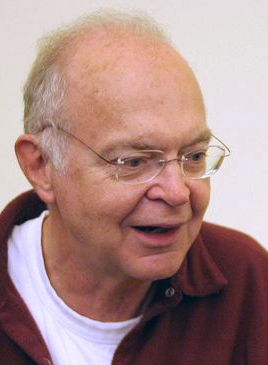
\includegraphics[width=1.7cm]{images/Knuth}}}%
\ghost{\raisebox{-5mm}{\textcolor{devilscss}{\tiny Don Knuth, 2005}}}%
\ghost{\raisebox{-8mm}{\textcolor{devilscss}{\tiny CC-By-SA 2.5}}}%
\ghost{\raisebox{-11mm}{\textcolor{devilscss}{\tiny (c) J. Appelbaum}}}\hspace{1.7cm}
\begin{minipage}{8.3cm}
In der Praxis hilft eine Verallgemeinerung von DCFGs:\\
\redalert{Grammatiken mit endlicher Vorschau} (Look\-ahead).\medskip

\footnotesize
\emph{~~Idee:}
\begin{itemize}
\item Wort wird von links nach rechts gelesen
\item Grammatikregeln werden rückwärts angewendet, um Teile des gelesenen Worts zu reduzieren
% \item Indirekt entstehen \textcolor<3->{darkred}{R}echtsableitungen (da man von links reduziert)
\item Die Wahl der Grammatikregel hängt nur vom schon gelesenen Wort und von bis zu {$k$} weiteren
Symbolen ab (Vorschau)
\end{itemize}\end{minipage}\medskip

Grammatiken, die das erlauben, sind vom Typ $\Slang{LR}(k)$, wobei $\Slang{LR}(0)$ (keine Vorschau) DCFGs sind.
}

\end{frame}

\begin{frame}\frametitle{Abschlusseigenschaften (1)}

Wir wissen bereits, dass deterministische Typ-2-Sprachen unter Komplement abgeschlossen sind.
\medskip\pause

Für Schnitte gilt das allerdings nicht:
\medskip

\theobox{Satz: Deterministische Typ-2-Sprachen sind nicht unter Schnitten abgeschlossen.}\pause

\emph{Beweis:} Der Beweis für Typ-2-Sprachen funktioniert auch hier.
Die Sprachen
\begin{align*}
\Slangsub{L}{1}&= \{\Sterm{a}^i\Sterm{b}^i\Sterm{c}^k\mid i\geq 0, k\geq 0\}\\
\Slangsub{L}{2}&= \{\Sterm{a}^i\Sterm{b}^k\Sterm{c}^k\mid i\geq 0, k\geq 0\}.
\end{align*}
sind deterministisch kontextfrei (Übung: Geben Sie entsprechende DPDAs an). Ihr Schnitt $\Slangsub{L}{1}\cap\Slangsub{L}{2}=\{\Sterm{a}^i\Sterm{b}^i\Sterm{c}^i\mid i\geq 0\}$ ist dagegen nicht einmal kontextfrei.\qed

\end{frame}

\begin{frame}\frametitle{Abschlusseigenschaften (2)}

Der Nichtabschluss unter Schnitten hat weitere Konsequenzen:\medskip

\theobox{Satz: Deterministische Typ-2-Sprachen sind nicht unter Vereinigung abgeschlossen.}\pause

\emph{Beweis:} Angenommen sie wären unter Vereinigung abgeschlossen, dann
wären sie auch unter Schnitten abgeschlossen, da sie bereits unter Komplement abgeschlossen sind (De Morgan).
Widerspruch.
\qed

\end{frame}

\begin{frame}\frametitle{Abschlusseigenschaften (3)}

Bei anderen Operationen sieht es nicht besser aus:\medskip

\theobox{Satz: Deterministische Typ-2-Sprachen sind nicht unter Konkatenation oder Kleene-Stern abgeschlossen.}\pause

\emph{Beweisidee:} Vereinigungen kann man deterministisch machen, indem man einer der Alternativen ein Markierungszeichen $\Sterm{X}$ vorschaltet, das ansonsten nie am Anfang des Wortes auftauchen darf. Falls man die Sprache dann aber an die (deterministische Sprache) $\Sterm{X}^*$ anhängt, ist die Markierung nicht mehr als Entscheidungshilfe nutzbar.
Die Idee beim Stern ist ähnlich.\qed
\bigskip

\emph{Zusammenfassung:} Deterministische Typ-2-Sprachen sind 
abgeschlossen unter Komplement, aber nicht unter Vereinigung, Schnitt, Konkatenation oder Stern.

\end{frame}

% \begin{frame}\frametitle{Abschlusseigenschaften (4)}
% 
% Eventuell Kommentar zum Schnitt mit regulären Sprachen
% 
% \end{frame}

\sectionSlide{Entscheidungsprobleme auf kontextfreien Sprachen}

\begin{frame}\frametitle{Rückblick Entscheidungsprobleme}

Für reguläre Sprachen haben wir eine Reihe von Problemstellungen kennengelernt:
\begin{itemize}
\item \alert{Leerheitsproblem:} Ist die beschriebene Sprache $\emptyset$?
\item \alert{Inklusionsproblem:} Ist eine beschriebene Sprache Teilmenge einer anderen?
\item \alert{Äquivalenzproblem:} Wird durch zwei Beschreibungen die selbe Sprache gegeben?
\item \alert{Endlichkeitsproblem:} Ist die beschriebene Sprache endlich?
\item \alert{Universalitätsproblem:} Ist die beschriebene Sprache $\Sigma^*$?
\end{itemize}

Dabei könnten Sprachen durch verschiedene Beschreibungen gegeben sein (Automaten, Grammatiken, \ldots)
\medskip

\footnotesize
\textcolor{devilscss}{Zudem gibt es freilich das Wortproblem\\ (für [D]CFGs bereits besprochen)}

\end{frame}

\begin{frame}\frametitle{Meistens unentscheidbar}

Viele interessante Fragen sind leider im Allgemeinen nicht durch Algorithmen lösbar:\medskip

\theobox{Satz: Inklusion, Äquivalenz und Universalität von CFGs ist unentscheidbar.}

(ohne Beweis, da wir noch gar nicht über Entscheidbarkeit gesprochen haben \ldots)
\medskip\pause

Einiges ist aber doch machbar:

\theobox{Satz: Leerheit und Endlichkeit einer CFG sind entscheidbar.}\medskip

Diese Ergebnisse gelten ebenso, wenn PDAs statt CFGs gegeben sind, da wir diese ja in CFGs umwandeln können.

\end{frame}

\begin{frame}\frametitle{Leerheit entscheiden}

\theobox{Satz: Die Leerheit einer CFG ist entscheidbar.}

\emph{Beweis:} Man markiert Variablen mit folgender Prozedur:
\begin{itemize}
\item Markiere alle Variablen, welche direkt in ein Wort aus Terminalzeichen umgeschrieben werden können
\item Markiere rekursiv alle Variablen, welche in ein Wort aus Terminalzeichen und markierten Variablen umgeschrieben werden können
\end{itemize}
Die Sprache ist genau dann nicht leer wenn bei diesem Verfahren das Startsymbol markiert wird.\qed

\end{frame}

\begin{frame}\frametitle{Endlichkeit entscheiden}

\theobox{Satz: Endlichkeit der Sprache $\Slang{L}(G)$ einer CFG $G$ ist entscheidbar.}\pause

\emph{Beweis:} Sei $n$ die Zahl aus dem Pumpinglemma (also $2^{|V|}$).\pause
\begin{itemize}
\item Wenn es ein Wort $z\in\Slang{L}(G)$ mit $n\leq|z|<2n$ gibt, dann ist $\Slang{L}(G)$
unendlich (da man das Pumpinglemma auf $z$ anwenden \ghost{kann).} \pause
\item Wenn $\Slang{L}(G)$ unendlich ist, dann gibt es ein Wort $z\in\Slang{L}(G)$ mit $n\leq|z|<2n$ \pause
(Beweis: Es muss Wörter mit mehr als $n$ Zeichen geben. \pause Sei $z$ ein kürzestes Wort dieser Art. \pause
Laut Pumpinglemma ist $z=uvwxy$ mit $|vx|<n$ und $uv^0wx^0y=uwy\in\Slang{L}(G)$. \pause Da $uwy$ kürzer ist als $z$
muss gelten $|uwy|<n$. \pause Daraus folgt $|z|=|uwy|+|vx|<2n$.)\pause
\end{itemize}
Das heißt, wir müssen nur testen, ob es so ein Wort $z\in\Slang{L}(G)$ mit $n\leq|z|<2n$ gibt.
Das kann man (Brute Force) für alle Wörter dieser Länge tun (da das Wortproblem lösbar ist). \qed

{\tiny(Es gibt effizientere Verfahren, aber dieses ist das einfachste für den Beweis.)}

\end{frame}

\begin{frame}\frametitle{Alles unentscheidbar}

Viele weitere interessante Fragen sind leider ebenfalls unentscheidbar:

\begin{itemize}
\item \alert{Regularität:} Ist die durch eine CFG gegebene Sprache regulär?
\item \alert{Mehrdeutigkeit:} Ist eine gegebene CFG mehrdeutig oder nicht?
\item \alert{Determinisierbarkeit:} Ist die durch eine CFG gegebene Sprache deterministisch?\footnote{Aber, wie zuvor angemerkt: man kann entscheiden, ob eine gegebene CFG bereits deterministisch ist
(wenn sie es nicht ist, dann bedeutet das aber nicht, dass es keine äquivalente DCFG geben könnte).}
\item \alert{Schnittproblem:} Haben zwei gegebene Sprachen gemeinsame Wörter?
\end{itemize}


\end{frame}

\begin{frame}\frametitle{Entscheidungsprobleme für DPDAs}

Die Situation ist etwas besser bei DPDAs:
\bigskip

\begin{tabular}{rl}
Leerheit & \textcolor{darkgreen}{entscheidbar} {\tiny(wie bei CFGs)}\\
Endlichkeit & \textcolor{darkgreen}{entscheidbar} {\tiny(wie bei CFGs)} \\\pause
Universalität & \pause\textcolor{darkgreen}{entscheidbar} {\tiny(entspricht Leerheit des Komplements)}\\\pause
Regularität & \textcolor{darkgreen}{entscheidbar}\\[-1.5ex]
	& {\tiny (Stearns: A Regularity Test for Pushdown Machines, 1967)}\pause\\[-1ex]
Inklusion  & \textcolor{darkred}{unentscheidbar}\\[-1.5ex]
	& {\tiny (Ginsburg \& Greibach: Deterministic context-free languages, 1966)}\pause\\[-1ex]
Schnitt & \pause\textcolor{darkred}{unentscheidbar} {\tiny(wie Inklusion, da wir Komplemente haben)}\\\pause
Äquivalenz  \pause& \textcolor{darkgreen}{entscheidbar!}\\[-1.5ex]
	& {\tiny (S\'{e}nizergues: L(A)=L(B)? decidability results from complete formal systems, 2001;}\\[-1.5ex]
	& {\tiny ~komplexes Verfahren ohne Komplexitätsschranken; Ergebnis bekannt seit 1997)}\\[-1ex]
\end{tabular}\bigskip

(Mehrdeutigkeit und Determinisierbarkeit sind bei DPDAs trivial)

\end{frame}

\begin{frame}\frametitle{Übersicht}

\begin{tabular}{rll}
 & \emph{CFG} & \emph{DPDA}\\
Wortproblem
	& in $O(|w|^3)$
	& in $O(|w|)$\\[1ex]
Leerheit 
	& \textcolor{darkgreen}{entscheidbar}
	& \textcolor{darkgreen}{entscheidbar}\\
Endlichkeit
	& \textcolor{darkgreen}{entscheidbar}
	& \textcolor{darkgreen}{entscheidbar}\\
Universalität
	& \textcolor{darkred}{unentscheidbar}
	& \textcolor{darkgreen}{entscheidbar}\\[1ex]
Inklusion
	& \textcolor{darkred}{unentscheidbar}
	& \textcolor{darkred}{unentscheidbar}\\
Schnitt
	& \textcolor{darkred}{unentscheidbar}
	& \textcolor{darkred}{unentscheidbar}\\
Äquivalenz
	& \textcolor{darkred}{unentscheidbar}
	& \textcolor{darkgreen}{entscheidbar}\\[1ex]
Regularität
	& \textcolor{darkred}{unentscheidbar}
	& \textcolor{darkgreen}{entscheidbar}\\
Mehrdeutigkeit
	& \textcolor{darkred}{unentscheidbar}
	& \textcolor{gray}{trivial}\\
Determinisierbarkeit 
	& \textcolor{darkred}{unentscheidbar}
	& \textcolor{gray}{trivial}\\
\end{tabular}

\end{frame}

\sectionSlide{Rechnen mit Typ 1 und Typ 0}

\begin{frame}\frametitle{Wortprobleme jenseits von Typ 2}

Wir haben gesehen:
\begin{itemize}
\item endliche Automaten erkennen Typ-3-Sprachen
\item endliche Automaten + Kellerspeicher erkennen Typ-2-Sprachen
\end{itemize}\vspace{-5mm}

\narrowcentering{%
\begin{tikzpicture}[
	scale=0.50,
	decoration=penciline, decorate
]
% \path[use as bounding box] (-3.2,0) rectangle (3.5,-5); % add "draw" to see it
% \draw[help lines] (0,0) grid (5,5);
\pgfmathsetseed{5712}
%
\node (inlabel) [circle,draw=none,inner sep=1pt] at (2,0.5) {\alert{Eingabewort}};
\draw[decorate,line width=0.3mm] (-1,0) -- (4.5,0);
\draw[decorate,line width=0.3mm] (-1,-1) -- (4.5,-1);
\foreach \x in {0,...,4} {
	\draw[decorate,line width=0.3mm] (\x-1,0) -- (\x-1,-0.9);
	\node (s\x) [circle,draw=none,inner sep=1pt] at (\x-0.5,-0.5) {\ifthenelse{\x<4}{\Sterm{a}}{\Sterm{b}}};
}
\draw[decorate,line width=0.3mm] (4,0) -- (4,-0.9);
\node (dots) [circle,draw=none,inner sep=1pt] at (5.1,-0.5) {$\cdots$};

\draw[decorate,line width=0.3mm] (5.5,0) -- (6,0) -- (6,-0.9) -- (5.5,-0.9) ;
% \draw[decorate,line width=0.3mm] (6,0) -- (6,-0.9);

\draw[fill=none,decorate,line width=0.3mm]
	(2,-3) -- (6,-3) -- (6,-7) -- (2,-7) -- cycle;
\node (falabel) [circle,draw=none,inner sep=1pt,align=left] at (4,-5) {Endliche\\Steuerung};
\draw[fill=none,decorate,line width=0.4mm,darkblue,->]
	(4,-3) -- (4,-2) -- (1.5,-2) -> (1.5,-1);

\node[rectangle,align=center,draw,line width=0.3mm,decorate, minimum width=8mm, minimum height=8mm] (state) at (8, -6) {$q$};
\draw[fill=none,decorate,line width=0.4mm,darkblue,->]
	(6,-6) -> (state.180);
\node (qlabel) [circle,draw=none,inner sep=1pt] at (11.5,-6) {\footnotesize\alert{Zustandsvariable}};

% \node[cloud, cloud puffs=15.7, cloud ignores aspect, minimum width=4cm, minimum height=1cm, align=center, draw,line width=0.3mm] (memory) at (11, -1) {\alert{zusätzlicher}\\\alert{Speicher}};

\draw[fill=none,decorate,line width=0.3mm] (9,0) -- (9,-4);
\draw[fill=none,decorate,line width=0.3mm] (10,0) -- (10,-4);
\draw[fill=none,decorate,line width=0.3mm] (8.5,-4) -- (10.5,-4);
\foreach \y in {0,...,-3} {
	\draw[fill=none,decorate,line width=0.3mm] (9,\y) -- (10,\y);
	\node (k\y) [circle,draw=none,inner sep=1pt] at (9.5,\y-0.5) {\ifthenelse{\y<-1}{\Snterm{A}}{\Snterm{B}}};
}
\draw[fill=none,decorate,line width=0.4mm,darkblue,->]
	(6,-3.5) -- (7.5,-3.5) -- (7.5,-0.5) -> (9,-0.5);
\node (stacklabel) [circle,draw=none,inner sep=1pt] at (11.5,-2.5) {\alert{Keller}};
\end{tikzpicture}}
\vspace{-5mm}

\redalert{Für Typ 1 und Typ 0 benötigen wir mehr als das -- aber was?}

\end{frame}

\begin{frame}\frametitle{Berechnungsmodelle nach Kellerautomaten?}

\emph{Beobachtung:} Auch jenseits von Typ 2 kann man Wortprobleme algorithmisch lösen.
\medskip

\examplebox{Beispiel: Die Sprache $\{\Sterm{a}^i\Sterm{b}^i\Sterm{c}^i\mid i\geq 0\}$ ist nicht
kontextfrei, wird also von keinem PDA erkannt. Dennoch wäre es nicht sehr schwer, ein 
Programm in einer beliebigen Programmiersprache zu schreiben, welches feststellt, ob eine Eingabe diese
Form hat.}\pause

\emph{Aber:} Praktische Programmiersprachen eignen sich schlecht als allgemeine Berechnungsmodelle, da sie viel zu kompliziert sind.\bigskip

$\leadsto$ Wir wollen lieber unser Automatenmodell erweitern

\end{frame}

\begin{frame}\frametitle{Jenseits PDAs (1)\visible<2->{: Mehr Stapel}}

\anybox{purple}{%
Die Haupteinschränkung von Kellerautomaten war das eingeschränkte Speichermodell. Wir könnte man das erweitern?}%
\pause\smallskip

\begin{itemize}
\item Man könnte statt eines Stapelspeichers zwei (oder mehr) Stapel verwenden
\item Automatenübergänge werden zum Zugriff auf weitere Stapel entsprechend erweitert
\end{itemize}%
\vspace{-3.5ex}

\narrowcentering{%
\begin{tikzpicture}[
	scale=0.50,
	decoration=penciline, decorate
]
% \path[use as bounding box] (-3.2,0) rectangle (3.5,-5); % add "draw" to see it
% \draw[help lines] (0,0) grid (5,5);
\pgfmathsetseed{5712}
%
\node (inlabel) [circle,draw=none,inner sep=1pt] at (2,0.5) {\alert{Eingabewort}};
\draw[decorate,line width=0.3mm] (-1,0) -- (4.5,0);
\draw[decorate,line width=0.3mm] (-1,-1) -- (4.5,-1);
\foreach \x in {0,...,4} {
	\draw[decorate,line width=0.3mm] (\x-1,0) -- (\x-1,-0.9);
	\node (s\x) [circle,draw=none,inner sep=1pt] at (\x-0.5,-0.5) {\ifthenelse{\x<4}{\Sterm{a}}{\Sterm{b}}};
}
\draw[decorate,line width=0.3mm] (4,0) -- (4,-0.9);
\node (dots) [circle,draw=none,inner sep=1pt] at (5.1,-0.5) {$\cdots$};

\draw[decorate,line width=0.3mm] (5.5,0) -- (6,0) -- (6,-0.9) -- (5.5,-0.9) ;
% \draw[decorate,line width=0.3mm] (6,0) -- (6,-0.9);

\draw[fill=none,decorate,line width=0.3mm]
	(2,-3) -- (6,-3) -- (6,-7) -- (2,-7) -- cycle;
\node (falabel) [circle,draw=none,inner sep=1pt,align=left] at (4,-5) {Endliche\\Steuerung};
\draw[fill=none,decorate,line width=0.4mm,darkblue,->]
	(4,-3) -- (4,-2) -- (1.5,-2) -> (1.5,-1);

\node[rectangle,align=center,draw,line width=0.3mm,decorate, minimum width=8mm, minimum height=8mm] (state) at (8, -6) {$q$};
\draw[fill=none,decorate,line width=0.4mm,darkblue,->]
	(6,-6) -> (state.180);
\node (qlabel) [circle,draw=none,inner sep=1pt] at (11.5,-6) {\footnotesize\alert{Zustandsvariable}};

% \node[cloud, cloud puffs=15.7, cloud ignores aspect, minimum width=4cm, minimum height=1cm, align=center, draw,line width=0.3mm] (memory) at (11, -1) {\alert{zusätzlicher}\\\alert{Speicher}};

\draw[fill=none,decorate,line width=0.3mm] (11,0) -- (11,-4);
\draw[fill=none,decorate,line width=0.3mm] (12,0) -- (12,-4);
\draw[fill=none,decorate,line width=0.3mm] (8.5,-4) -- (12.5,-4);
\foreach \y in {0,...,-3} {
	\draw[fill=none,decorate,line width=0.3mm] (11,\y) -- (12,\y);
	\node (k\y) [circle,draw=none,inner sep=1pt] at (11.5,\y-0.5) {\ifthenelse{\y<-1}{\Snterm{A}}{\Snterm{B}}};
}

\draw[fill=none,decorate,line width=0.3mm] (9,-1) -- (9,-4);
\draw[fill=none,decorate,line width=0.3mm] (10,-1) -- (10,-4);
\foreach \y in {-1,...,-3} {
	\draw[fill=none,decorate,line width=0.3mm] (9,\y) -- (10,\y);
	\node (k\y) [circle,draw=none,inner sep=1pt] at (9.5,\y-0.5) {\ifthenelse{\y<-2}{\Snterm{B}}{\Snterm{A}}};
}

\draw[fill=none,decorate,line width=0.4mm,darkblue,->]
	(6,-3.5) -- (7.5,-3.5) -- (7.5,-0.5) -> (11,-0.5);
\draw[fill=none,decorate,line width=0.4mm,darkblue,->]
	(7.5,-1.5) -- (9,-1.5);
\node (stacklabel) [circle,draw=none,inner sep=1pt] at (13.5,-2.5) {\alert{Keller}};
\end{tikzpicture}}

\end{frame}

\begin{frame}\frametitle{Jenseits PDAs (2)\visible<2->{: \ghost{"`Warteschlangenautomaten"'}}}

\anybox{purple}{%
Die Haupteinschränkung von Kellerautomaten war das eingeschränkte Speichermodell. Wir könnte man das erweitern?}%
\pause\smallskip

\begin{itemize}
\item Man könnte statt eines Stapelspeichers eine Warteschlange (Queue) verwenden
$\leadsto$ first-in/first-out (FIFO)
% \item Die Hauptoperationen sind dann \texttt{enqueue} und \texttt{dequeue}
\item Definition fast genau wie bei PDAs, aber mit \texttt{enqueue}/\texttt{dequeue} statt \texttt{push}/\texttt{pop}
\end{itemize}%
\vspace{-3.5ex}

\narrowcentering{%
\begin{tikzpicture}[
	scale=0.50,
	decoration=penciline, decorate
]
% \path[use as bounding box] (-3.2,0) rectangle (3.5,-5); % add "draw" to see it
% \draw[help lines] (0,0) grid (5,5);
\pgfmathsetseed{5712}
%
\node (inlabel) [circle,draw=none,inner sep=1pt] at (2,0.5) {\alert{Eingabewort}};
\draw[decorate,line width=0.3mm] (-1,0) -- (4.5,0);
\draw[decorate,line width=0.3mm] (-1,-1) -- (4.5,-1);
\foreach \x in {0,...,4} {
	\draw[decorate,line width=0.3mm] (\x-1,0) -- (\x-1,-0.9);
	\node (s\x) [circle,draw=none,inner sep=1pt] at (\x-0.5,-0.5) {\ifthenelse{\x<4}{\Sterm{a}}{\Sterm{b}}};
}
\draw[decorate,line width=0.3mm] (4,0) -- (4,-0.9);
\node (dots) [circle,draw=none,inner sep=1pt] at (5.1,-0.5) {$\cdots$};

\draw[decorate,line width=0.3mm] (5.5,0) -- (6,0) -- (6,-0.9) -- (5.5,-0.9) ;
% \draw[decorate,line width=0.3mm] (6,0) -- (6,-0.9);

\draw[fill=none,decorate,line width=0.3mm]
	(2,-3) -- (6,-3) -- (6,-7) -- (2,-7) -- cycle;
\node (falabel) [circle,draw=none,inner sep=1pt,align=left] at (4,-5) {Endliche\\Steuerung};
\draw[fill=none,decorate,line width=0.4mm,darkblue,->]
	(4,-3) -- (4,-2) -- (1.5,-2) -> (1.5,-1);

\node[rectangle,align=center,draw,line width=0.3mm,decorate, minimum width=8mm, minimum height=8mm] (state) at (8, -6) {$q$};
\draw[fill=none,decorate,line width=0.4mm,darkblue,->]
	(6,-6) -> (state.180);
\node (qlabel) [circle,draw=none,inner sep=1pt] at (11.5,-6) {\footnotesize\alert{Zustandsvariable}};

% \node[cloud, cloud puffs=15.7, cloud ignores aspect, minimum width=4cm, minimum height=1cm, align=center, draw,line width=0.3mm] (memory) at (11, -1) {\alert{zusätzlicher}\\\alert{Speicher}};

\draw[fill=none,decorate,line width=0.3mm] (9,0) -- (14,0);
\draw[fill=none,decorate,line width=0.3mm] (9,-1) -- (14,-1);
\draw[fill=none,decorate,line width=0.3mm] (9,0) -- (9,-1);
\foreach \y in {10,...,14} {
	\draw[fill=none,decorate,line width=0.3mm] (\y,0) -- (\y,-0.9);
	\node (k\y) [circle,draw=none,inner sep=1pt] at (\y-0.5,-0.5) {\ifthenelse{\y<12}{\Snterm{A}}{\Snterm{B}}};
}
\draw[fill=none,decorate,line width=0.4mm,darkblue,->]
	(6,-3.5) -- (7.5,-3.5) -- (7.5,-0.5) -> (9,-0.5);
\node (stacklabel) [circle,draw=none,inner sep=1pt] at (11.5,-1.5) {\alert{Warteschlange}};
\end{tikzpicture}}

\end{frame}

\begin{frame}\frametitle{Jenseits PDAs (3)\visible<2->{: Zählerautomaten}}

\anybox{purple}{%
Die Haupteinschränkung von Kellerautomaten war das eingeschränkte Speichermodell. Wir könnte man das erweitern?}%
\pause\smallskip

\begin{itemize}
\item Man könnte statt eines Stapelspeichers (endlich viele) Speicherplätze für natürliche Zahlen einführen
\item Automatenübergänge könnten einzelne Variablen inkrementieren, dekrementieren, auf Gleichheit mit $0$ testen, \ghost{\ldots}
\end{itemize}%
\vspace{-3.5ex}

\narrowcentering{%
\begin{tikzpicture}[
	scale=0.50,
	decoration=penciline, decorate
]
% \path[use as bounding box] (-3.2,0) rectangle (3.5,-5); % add "draw" to see it
% \draw[help lines] (0,0) grid (5,5);
\pgfmathsetseed{5712}
%
\node (inlabel) [circle,draw=none,inner sep=1pt] at (2,0.5) {\alert{Eingabewort}};
\draw[decorate,line width=0.3mm] (-1,0) -- (4.5,0);
\draw[decorate,line width=0.3mm] (-1,-1) -- (4.5,-1);
\foreach \x in {0,...,4} {
	\draw[decorate,line width=0.3mm] (\x-1,0) -- (\x-1,-0.9);
	\node (s\x) [circle,draw=none,inner sep=1pt] at (\x-0.5,-0.5) {\ifthenelse{\x<4}{\Sterm{a}}{\Sterm{b}}};
}
\draw[decorate,line width=0.3mm] (4,0) -- (4,-0.9);
\node (dots) [circle,draw=none,inner sep=1pt] at (5.1,-0.5) {$\cdots$};

\draw[decorate,line width=0.3mm] (5.5,0) -- (6,0) -- (6,-0.9) -- (5.5,-0.9) ;
% \draw[decorate,line width=0.3mm] (6,0) -- (6,-0.9);

\draw[fill=none,decorate,line width=0.3mm]
	(2,-3) -- (6,-3) -- (6,-7) -- (2,-7) -- cycle;
\node (falabel) [circle,draw=none,inner sep=1pt,align=left] at (4,-5) {Endliche\\Steuerung};
\draw[fill=none,decorate,line width=0.4mm,darkblue,->]
	(4,-3) -- (4,-2) -- (1.5,-2) -> (1.5,-1);

\node[rectangle,align=center,draw,line width=0.3mm,decorate, minimum width=8mm, minimum height=8mm] (state) at (8, -6) {$q$};
\draw[fill=none,decorate,line width=0.4mm,darkblue,->]
	(6,-6) -> (state.180);
\node (qlabel) [circle,draw=none,inner sep=1pt] at (11.5,-6) {\footnotesize\alert{Zustandsvariable}};

% \node[cloud, cloud puffs=15.7, cloud ignores aspect, minimum width=4cm, minimum height=1cm, align=center, draw,line width=0.3mm] (memory) at (11, -1) {\alert{zusätzlicher}\\\alert{Speicher}};

\draw[fill=none,decorate,line width=0.3mm] (9,0) -- (9,-3);
\draw[fill=none,decorate,line width=0.3mm] (10,0) -- (10,-3);
\foreach \y in {0,...,-3} {
	\draw[fill=none,decorate,line width=0.3mm] (9,\y) -- (10,\y);
}
\node (k1) [circle,draw=none,inner sep=1pt] at (9.55,-0.5) {\Snterm{17}};
\node (k2) [circle,draw=none,inner sep=1pt] at (9.55,-1.5) {\Snterm{42}};
\node (k3) [circle,draw=none,inner sep=1pt] at (9.55,-2.5) {\Snterm{23}};

\draw[fill=none,decorate,line width=0.4mm,darkblue,->]
	(6,-3.5) -- (7.5,-3.5) -- (7.5,-0.5) -> (9,-0.5);
\draw[fill=none,decorate,line width=0.4mm,darkblue,->] (7.5,-1.5) -> (9,-1.5);
\draw[fill=none,decorate,line width=0.4mm,darkblue,->] (7.5,-2.5) -> (9,-2.5);
\node (stacklabel) [circle,draw=none,inner sep=1pt] at (11.5,-1.5) {\alert{Zähler}};
\end{tikzpicture}}

\end{frame}

\begin{frame}\frametitle{Jenseits PDAs (4): Programme statt \ghost{Automaten}}

Eventuell könnte man auch vom Automatenmodell abweichen und stattdessen eine
einfache Programmiersprache definieren.\pause
\medskip

\emph{Einfache Ausdrucksmittel:}
\begin{itemize}
\item \alert{Variablen}, die Zahlen speichern können
\item \alert{Wertezuweisungen}, die Variablen das Ergebnis eines Ausdrucks (z.B. aus $+$, $-$, Variablen, Zahlen) zuweisen
\item \alert{Schleifen} der Form \Scode{while} $x\neq 0$ \Scode{do:} \ldots
\end{itemize}
$\leadsto$ Sogenannte \redalert{WHILE-Programme}\pause
\bigskip

Statt \Scode{while} könnte man auch \Scode{if} und \Scode{goto} einführen\\
$\leadsto$ Sogenannte \redalert{GOTO-Programme}

\end{frame}

\begin{frame}\frametitle{Viele mögliche Wege}

\emph{Bisher gesammelte Ideen:}
\begin{itemize}
\item PDAs mit zwei Stapeln
\item PDAs mit einer noch größeren Zahl an Stapeln
\item Warteschlangenautomaten
\item Zählerautomaten
\item WHILE-Programme
\item GOTO-Programme
\end{itemize}

Man kann jedes dieser Berechnungsmodelle formal definieren \ldots\medskip\pause

Es ergeben sich daher viele Fragen \ldots

\anybox{purple}{Welche Sprachklasse können diese Modelle jeweils erkennen?}\pause

\ldots aber immer wieder die gleiche Antwort\pause:\\[1ex]
\narrowcentering{{\Large\textcolor{purple}{Genau die Typ-0-Sprachen.}}}

% Die Antwort lautet: {\Large\redalert{genau die Typ-0-Sprachen}} (in jedem der Modelle)

% \anybox{darkred}{Die Typ-0-Sprachen}

\end{frame}

\begin{frame}\frametitle{Zusammenfassung und Ausblick}

\redalert{Deterministische Typ-2-Sprachen} sind praktisch wichtig, da effizient parsebar 
\bigskip

Viele \redalert{Fragestellungen für Typ-2-Sprachen} sind unentscheidbar, wobei deterministische Sprachen noch etwas mehr erlauben
\bigskip

\redalert{Zahlreiche naheliegende Erweiterungen von PDAs} führen alle zur gleichen Ausdrucksstärke (Typ 0)
\bigskip

\anybox{yellow}{
Offene Fragen:
\begin{itemize}
\item Welches Berechnungsmodell sollen wir nun verwenden?
\item Wenn alle Modelle Typ 0 liefern, was ist dann mit Typ 1?
\item Unterscheiden sich Typ 0 und Typ 1 überhaupt?
\end{itemize}
}

\end{frame}


\end{document}